\section{Software Implementation (GLaRe)}\label{sec:software}

% name it implemententation maybe?

The CoLLaRe framework is implemented in our \proglang{R} package called \pkg{GLaRe}.
The main function in the \pkg{GLaRe} package is \texttt{GLaRe()}, which computes and summarizes the cross-validated distribution of information loss and implements the CoLLaRe framework to compute the qualifying dimension for choice of $\alpha$ and $\epsilon$.
A sample call to the \texttt{GLaRe()} function is presented in Listing 1.

\begin{lstlisting}[language=R, caption={Example call to the \texttt{GLaRe()} function.}]
mnist_pca <- GLaRe(mat = x_train,
                   latent_dim_from = 1,
                   latent_dim_to = 400,
                   latent_dim_by = 20,
                   attainment_rate = 0.95,
                   tolerance_level = 0.05,
                   learn = "pca",
                   verbose = TRUE)
\end{lstlisting}
The \texttt{GLaRe()} function computes full cross-validated distribution of information losses for a latent feature representation method defined by \texttt{learn}, on dataset stored in the matrix \texttt{mat}, across a range of latent feature dimensions defined by the grid of equally-spaced values from \texttt{latent\_dim\_from} to \texttt{latent\_dim\_by} in increments of \texttt{latent\_dim\_by}.
It computes whether the method achieve the qualifying criterion defined by \texttt{tolerance\_level} ($\epsilon$) and \texttt{attainment\_rate} ($\alpha$) for this range of latent feature dimensions and, if so, the learned latent feature representation at the qualifying dimension.
We describe the main features of the \texttt{GLaRe()} function in the following sections.

\subsection{Learning Functions}\label{sec:learning-functions}

The learning function is the main engine of \texttt{GlaRe()}.
The learning function takes as arguments a data matrix $\mathbf{X}$ and latent feature dimension $K$, and learns the encoding and decoding transformation functions $f_K$ and $f_K^{-1}$.
For example, the learning function in PCA computes the first $K$ eigenvectors of the empirical covariance matrix of $\mathbf{X}$, and $f_K$ and $f_K^{-1}$ comprise matrix multiplication by the first $K$ eigenvectors.
In contrast, for an autoencoder, $f_K$ and $f_K^{-1}$ are general functions that map to and from a $K$-dimensional latent space and are parametrized by flexible neural networks.
In \texttt{GLaRe()}, the learning function is defined by the \texttt{learn} argument. 
We provide three built-in learning functions that can be used, as well as the option to specify a bespoke, user-defined learning function:
\begin{enumerate}
    \item Setting \texttt{learn = "pca"} specifies a PCA representation. The eigenvectors are computed by the Singular Value Decomposition (SVD) algorithm. In cases where $N < T$ (e.g., the Glaucoma or Gels data) the latent feature dimension for PCA can be, at most, $N-1$. Hence the maximum latent feature dimension \texttt{latent\_dim\_to} is set to a default of $\min(N-1, T)$ when using PCA.
    \item Setting \texttt{learn = "dwt"} (or \texttt{learn = "dwt.2d"} for data on a 2-dimensional domain) specifies a thresholded wavelet representation. For encoding, the DWT is applied to $\mathbf{X}$ and the most important $K$ latent features (i.e., wavelet coefficients) are learned from the data and are retained. The decoding function then applies the inverse DWT to the retained features. Our implementation uses the \pkg{wavselim} \proglang{R} package \parencite{whitcher_waveslim_2024} which uses the Daubechies orthonormal compactly supported wavelet of length $8$ \parencite{daubechies_ten_1992}, least asymmetric family and uses periodic boundary conditions. Additional details are described in Appendix \ref{sec:wavelet-thresholding-algorithm}.
    \item Setting \texttt{learn = "ae"} specifies an autoencoder representation. We implement the autoencoder using the \pkg{keras} \proglang{R} package \parencite{kalinowski_keras_2024}. The encoder and decoder functions are parametrized by neural networks with a single hidden layer (defaulting to size $600$) and a rectified linear unit (ReLU) activation function.
    A linear activation function is used to map the hidden layer of the encoder to the latent space, and either a linear and sigmoid (default) activation function can be used to map from the hidden layer of the decoder back to the data space.
    By default, the autoencoder is trained for $100$ epochs using the ADAM stochastic gradient descent algorithm \parencite{kingma_adam_2017} to minimize either the mean squared error (default) or binary cross-entropy loss functions using a mini-batch size of $16$.
    \item Setting \texttt{learn = "user"} allows the user to specify their own latent feature representation method. With this setting, the user must supply the learning function for their method, that takes the data matrix $\mathbf{X}$ and the latent feature dimension $K$ as inputs and returns a list with two elements: functions named \texttt{Encode} and \texttt{Decode} implementing the learned encoding and decoding transformation functions $f_K$ and $f_K^{-1}$. 
    % \jsm{[MENTION THAT THE APPENDIX CONTAINS INSTRUCTS HOW THE USER CAN DEFINE THEIR OWN LEARNING FUNCTIONS FOR ANY DESIRED FEATURE REPRESENTATION APPROACH TO BE COMPATIBLE WITH GLARE.  ALSO PLAY UP IN THE INTRODUCTION/DISCUSSION HOW A FEATURE OF THIS METHOD IS ITS FORWARD COMPATABILITY WITH ANY POTENTIAL USER DEFINED FEATURE REPRESENTATION GIVEN THEIR LEARNING FUNCTION.  ALSO MENTION THE LEARNING FUNCTION MUST CONTAIN AN ENCODE AND DECODE STEP, AND OTHERWISE IN THE SUPPLEMENT BE SURE THE INSTRUCTIONS ARE SUFFICIENTLY DETAILED FOR USERS TO CONSTRUCT THEM.]}
\end{enumerate}

\subsection{Squared Correlation Loss}\label{sec:loss-functions}

In principle, any loss function can be used with \texttt{GLaRe()} and the package has been structured such that different loss functions can be used in future iterations.
The current implementation uses the complement of the squared correlation
$$
1- \rho^2 \left\{X_i (\mathbf{t}), \widehat{X}^{(K)}_{i} (\mathbf{t}) \right\} =
1 - \frac{\left[ \mathlarger{\sum}_{t = 1}^T{\bigg\{X_i (t) - \overline{X}_i \bigg\} \bigg\{ \widehat{X}_i^{(K)} (t) - \overline{\widehat{X}}_i^{(K)} \bigg\}} \right]^2}{\mathlarger{\sum}_{t = 1}^T \bigg\{X_i (t) - \overline{X}_i \bigg\}^2 \mathlarger{\sum}_{t = 1}^T \bigg\{ \widehat{X}_i^{(K)} (t) - \overline{\widehat{X}}_i^{(K)} \bigg\} ^2},
$$
where
$$
\overline{X}_i = \frac{1}{N} \sum_{t=1}^T X_i (t) \quad \text{and} \quad \overline{\widehat{X}}_i^{(K)} = \frac{1}{N} \sum_{t=1}^T \widehat{X}_i^{(K)} (t).
$$
The criterion $1- \rho^2$ is a relative measure, bounded between $0$ and $1$: $1- \rho^2 = 0$ indicates losslessness and $1- \rho^2 = 1$ indicates that no information is preserved by the latent feature representation method.
Employing a relative measure ensures that choices for the tolerance level $\epsilon$ are comparable across datasets that differ in scale and dimensionality.
In Appendix \ref{sec:squared-correlation}, we highlight connections between squared correlation, the Predicted Residual Sum of Squares (PRESS) loss and the scree plot for PCA.

\subsection{Cross-Validation Algorithm}

Given the learning function (Section \ref{sec:learning-functions}), the loss function (Section \ref{sec:loss-functions}), the data matrix $\mathbf{X}$ and a grid of values for $K$, \texttt{GLaRe()} implements a $k$-fold cross validation algorithm to estimate the individual generalization errors (Algorithm 1).
In principle, it is possible to employ leave-one-out cross validation by setting the number of folds to the number of observations $N$.
However, in most of our real-world applications we employ a non-exhaustive search (e.g., $5$ or $10$-fold cross-validation) due to computational considerations.
When a non-exhaustive search is used, variability is induced by splitting of the data into folds (i.e., the data rows are randomly shuffled and then divided into folds), so we recommend fixing the random seed before running \texttt{GLaRe()} so that results are reproducible.
It can also be useful to re-run \texttt{GLaRe()} using different seeds to assess the sensitivity of results to the random split and to decide whether to employ a more computationally intensive exhaustive search.

\subsection{Software Outputs}

The \texttt{GLaRe()} function computes and returns the cross-validated information loss for each individual observation in the dataset.
If the qualifying criterion is met for the range of latent feature dimensions, the final model is re-trained on the full dataset at the qualifying dimension and the encoding and decoding functions are returned as \proglang{R} functions called \texttt{Encode()} and \texttt{Decode()}.
A summary plot of this distribution is also returned by default by the \proglang{GLaRe()} function (Figure \ref{fig:glare-anatomy-plot}).
The overall, or average, cross-validated loss is displayed in yellow, with the analogous loss computed on the training data shown in green for comparison.
Then, different quantiles of the distribution of individual cross-validated losses are displayed to summarize the full distribution: the minimum and maximum are shown in blue and red, respectively, a user-specified quantile of the distribution (set by the \texttt{cvqlines} argument) is displayed in purple and the quantile of the distribution being used as the attainment rate $\alpha$ (defaulting to 0.95, i.e., the $95$th percentile) is displayed in light gray.
The corresponding value of the tolerance level $\epsilon$ is overlaid as gray dashed horizontal line, and hence the latent feature dimension (i.e., location on the $x$-axis) at which the two gray lines meet corresponds to the qualifying dimension.
The tolerance level $\epsilon$ and the qualifying dimension ($qd$) are marked in bold and italic typeface on the $y$ and $x$ axes, respectively.
The \texttt{GLaRe()} function also returns a heat-map as an alternative summary of the individual cross-validated loss distribution, and the package also contains wrapper functions to display a dot-plot of the full distribution of cross-validated losses, the ratio of training to cross-validated losses and the reconstructions of individual observations at the qualifying dimension. 
Further details of additional functionalities are provided in Appendix \ref{sec:additional-outputs}.

\begin{figure}
    \centering
    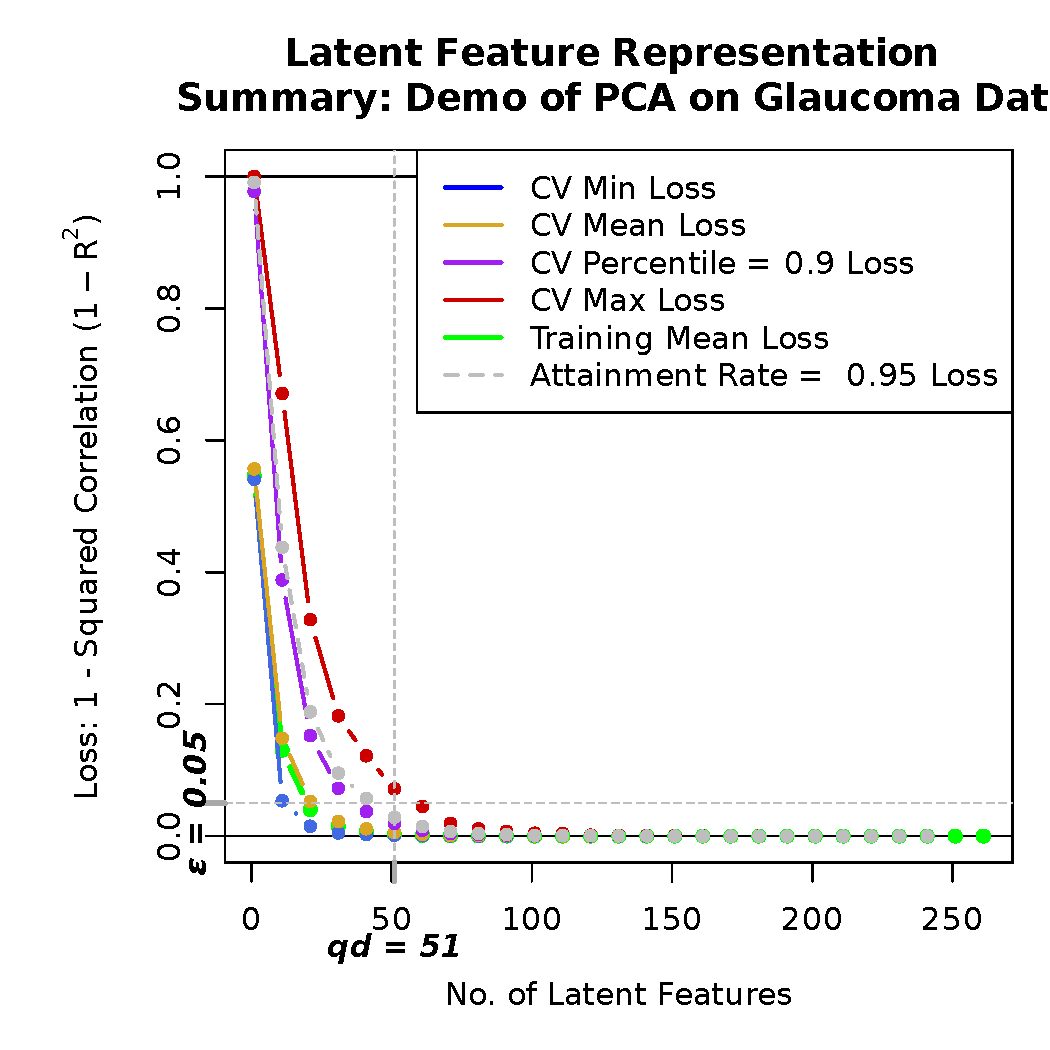
\includegraphics[width=0.5\linewidth]{figures/glare-anatomy-plot.pdf}
    \caption{The summary plot produced by \texttt{GlaRe()}, demonstrated on the Glaucoma dataset with PCA.}
    \label{fig:glare-anatomy-plot}
\end{figure}